\section{Préliminaires}

Nous supposerons ici que les notions de licence sur l'algèbre et la topologie sont acquises. Néanmoins, certains rappels sont effectués sur des notions essentielles pour le mémoire. Nous retrouverons également des notions complémentaires comme celles sur les homotopies.

\subsection{Topologie}
\subsubsection{Espace topologique}

\begin{definition}
On appelle \emph{espace topologique} un couple $(X,\mathcal{T})$, où $X$ est un ensemble et $\mathcal{T}$ une famille de parties de $X$, appelées \emph{ouverts} de $X$, vérifiant : \begin{enumerate}
    \item Les ensembles $\emptyset$ et $X$ sont des ouverts ;
    \item Toute réunion d'ouverts est un ouvert ;
    \item Une intersection finie d'ouverts est un ouvert.
\end{enumerate}
Les complémentaires des éléments de $\mathcal{T}$ sont appelés les \emph{fermés} de $E$.
\end{definition}

\begin{definition}
Un espace topologique $X$ est dit \emph{Hausdroff}, ou séparable, si pour tout couple d'éléments distincts $(x,y)\in X^2$, il existe $U\in\vois(x)$ et~$V\in~\vois(y)$, tel que $U\cap V=\emptyset$.
\end{definition}

Sauf mention contraire, nous désignerons tout au long du mémoire par $X$ un espace topologique, que nous appelons par abus de langage simplement espace.

\subsubsection{Connexité}

Intuitivement, un espace est dit connexe lorsqu'il est constituer d'un seul "morceau".

\begin{definition}
Un espace $X$ est dit \emph{connexe} s'il vérifie l'une des quatres propositions équivalentes : \begin{enumerate}
    \item L'espace n'est pas la réunion de deux ouverts non vides disjoints.
    \item L'espace n'est pas la réunion de deux fermés non vides disjoints.
    \item Les seuls éléments à la fois ouverts et fermés sont $\emptyset$ et $X$.
    \item Toute application continue de $X$ dans $\{0,1\}$ muni de la topologie discrète est constante.
\end{enumerate}

Pour un espace $X$, on appelle \emph{composante connexe} de $x$ dans $X$ la réunion de toutes les parties connexes contenant $x$. C'est la plus grande partie connexe contenant ce point, au sens de l'inclusion. L'ensemble des composantes connexes de $X$ forment une partition de l'espace $X$.

On dit que deux points sont \emph{connectés} s'ils appartiennent à la même composante connexe.
\end{definition}

En pratique, nous préférons utiliser une notions de connexité plus forte, qui est la connexité par arc.

\begin{definition}\label{def:path}
On appelle \emph{chemin} entre deux points $x_0$ et $x_1$ de $X$ une application $\gamma:[0,1]\to X$ continue, et telle que~$\gamma(0)=x_0$ et~$\gamma(1)=x_1$.
\end{definition}

\begin{remark}
Il est important de noter que les chemins ont une direction, donnée par l'application associée (de~$\gamma(0)$ vers $\gamma(1)$).
\end{remark}

\begin{exemple}
Sur l'espace euclidien $\bb{R}^n$, tout couple de point possède un chemin linéaire. Pour $x,y\in\bb{R}^n$, ce chemin est donné par l'application $t\mapsto (1-t)x+ty$.
\end{exemple}

\begin{definition}
Un espace $X$ est dit \emph{connexe par arc} si pour tout couples de points il existe un chemin reliant ces deux points.
\end{definition}

Nous verrons que les espaces connexes par arc sont connexes, mais l'exemple suivant nous montre que la réciproque n'est pas vraie.

\begin{exemple}
On considère le graphe de l'application $x\mapsto\sin\left(\frac{1}{x}\right)$ pour $x\in]0,1]$, auquel on ajoute son adhérence~$\{0\}\times[-1,1]$. Cet espace est connexe, mais nous ne pouvons pas créer de chemin entre un point du graphe et un point de l'adhérence. L'espace est alors non connexe par arc.
\begin{figure}[h]
    \centering
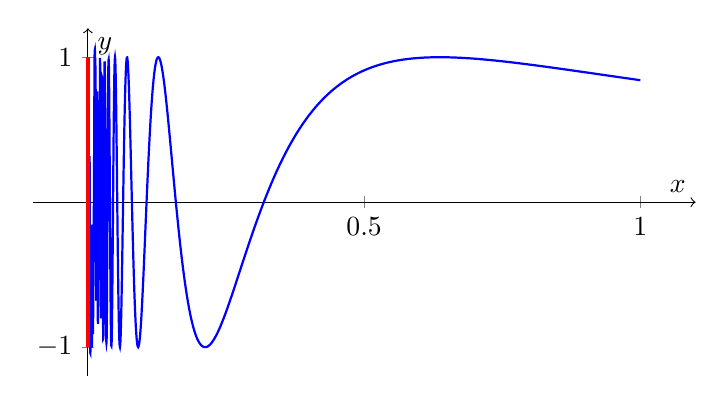
\begin{tikzpicture}
  \begin{axis}[
      axis lines=middle,
      xlabel={$x$},
      ylabel={$y$},
      domain=0.001:1, % éviter x=0
      samples=1000,
      xmin=-0.1, xmax=1.1,
      ymin=-1.2, ymax=1.2,
      width=10cm, height=6cm,
      xtick={0,0.5,1},
      ytick={-1,0,1},
      axis line style={->},
      smooth,
  ]
    % Courbe y = sin(1/x)
    \addplot[blue, thick] {sin(deg(1/x))};

    % Segment rouge de (0,-1) à (0,1)
    \addplot[red, very thick] coordinates {(0,-1) (0,1)};
  \end{axis}
\end{tikzpicture}
\label{tkz:non-path-connected}
\caption{Graphe de la courbe $x\mapsto\sin\left(\frac{1}{x}\right)$ (bleu) et son adhérence (rouge), connexe mais pas par arc}
\end{figure}
\end{exemple}

%\begin{exemple}
%Dans l'exemple qui suit la définition \ref{def:path}, nous avons vu qu'il existe un chemin pour tout couple de points de $\bb{R}^n$. On peut alors dire que l'espace euclidien $\bb{R}^n$ est connexe par arc.
%\end{exemple}

\begin{theorem}
Un espace connexe par arc est connexe.
\end{theorem}
La preuve de ce théorème se déroule par l'absurde, en supposant que l'espace est non connexe. L'idée est alors de définir l'espace comme deux ouverts disjoints non vides., et de considérer un chemin continue entre un point d'un ouvert vers l'autre. La contradiction découle du fait que $[0,1]$ n'est pas l'union de deux ouverts disjoints.

\subsubsection{Comparaisons d'espaces}

Il existe plusieurs moyens de comparer les espaces par des relations d'équivalences. Nous commençons par la relation la plus forte entre espaces : l'homéomorphisme.

\begin{definition}\label{def:homeo}
Un \emph{homéomorphisme} entre deux espaces $X$ et $Y$ est une application continue, inversible, et d'inverse continue. S'il existe un homéomorphisme entre $X$ et $Y$, on dit alors qu'ils sont \emph{homéomorphes}.
\end{definition}

\begin{exemple}
Le cercle $\s{1}$ auquel on supprime un point est homéomorphe à $\bb{R}$. De manière générale, la sphère~$\s{n}$ sur laquelle on supprime un point est homéomorphe à $\bb{R}^n$.

Le cercle est le carré sont homéomorphes. Intuitivement, il suffit soit d'arrondir les côtés du carré, soit de "pincer" quatres points du cercle.
\end{exemple}

La seconde relation est à propos de l'homotopie. Moins puissante que l'homéomorphisme, elle conserve toutefois la continuité dans l'espace ainsi que la connexité.

\begin{definition}\label{def:homotopy-spaces}
Deux applications $f_0,f_1:X\to Y$ sont dites \emph{homotopes} s'il existe une application continue~$F:X\times [0,1]\to Y$ telle que $F(0,x)=~f_0(x)$ et~$F(1,x)=f_1(x)$. Intuitivement, cela signifie qu'il existe une famille d'application~$f_t$, continue en $t$, permettant de passer de $f_0$ à $f_1$.
\end{definition}

De cette définition découle un cas particulier, lorsque le premier espace se rétracte en le second.

\begin{definition}\label{def:retracts}
Une \emph{déformation par rétraction} d'un espace $X$ en un sous-espace $A$ est une homotopie entre $f_0=id_X$, et $f_1(X)=A$, qui vérifie $f_t|_A=id_A$ pour tout $t\in[0,1]$. Nous appelons dans ce cas l'application $f_1$ une \emph{rétraction}.
\end{definition}

\begin{exemple}
Le disque $D^{n}$ se déforme par rétraction en un point.

\begin{figure}[H]
    \centering
    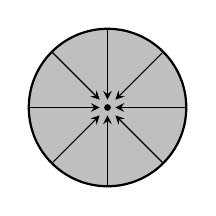
\begin{tikzpicture}
    \filldraw[lightgray] (0,0) circle(1cm);
    \filldraw[] (0,0) circle(1pt); %node[below right]{};
    \draw[thick] (0,0) circle(1cm);
    \draw[->, >=stealth] (1,0) -- (0.1, 0);
    \draw[->, >=stealth] (-1,0) -- (-0.1, 0);
    \draw[->, >=stealth] (0,1) -- (0,0.1);
    \draw[->, >=stealth] (0,-1) -- (0, -0.1);
    \draw[->, >=stealth] (1.4142135624/2,1.4142135624/2) -- (0.1, 0.1);
    \draw[->, >=stealth] (-1.4142135624/2,1.4142135624/2) -- (-0.1, 0.1);
    \draw[->, >=stealth] (1.4142135624/2,-1.4142135624/2) -- (0.1, -0.1);
    \draw[->, >=stealth] (-1.4142135624/2,-1.4142135624/2) -- (-0.1, -0.1);
    \end{tikzpicture}
    \caption{Rétraction par déformation du disque $D^2$ vers le point}
    \label{fig:def-retract-disk}
\end{figure}
\end{exemple}

\begin{definition}\label{def:homotopy-equiv}
Une application $f:X\to Y$ est une \emph{équivalence d'homotopie} s'il existe $g:Y\to X$ tel que~$fg\simeq id_Y$ et $gf\simeq id_X$. Dans ce cas, nous disons que $X$ et $Y$ sont homotopiquement équivalents, que l'on note $X\simeq Y$.
\end{definition}

\begin{exemple}
Pour une déformation par rétraction de $X$ vers $A$, avec $i:A\to X$ l'inclusion et $r:X\to A$ la rétraction, nous avons $ri\simeq id_A$ et $ir\simeq id_X$.
\end{exemple}

\subsection{Algèbre}

Sauf mention contraire, nous désignerons par $G$ un groupe, et $H$ un sous-groupe de $G$.

\subsubsection{Quotient}

\begin{definition}
On dit que le sous-groupe $H$ de $G$ est \emph{normal} s'il est stable par automorphisme intérieur, c'est à dire vérifiant pour tout $g\in G$ l'inclusion $gHg\inv\subset H$.
\end{definition}

Les sous-groupes normaux sont intéressants car permettent de pratiquer le quotient. Si un sous-groupe n'est pas normal pour un groupe, il peut l'être pour un sous-groupe.

\begin{definition}\label{def:normalizer}
Nous disons d'un élément $g$ qu'il \emph{normalise} $H$ s'il vérifie $gHg\inv=H$. L'ensemble des éléments qui normalisent~$H$ est appelé \emph{normalisateur} de $H$, noté~$N(H)$. Le normalisateur est le plus petit sous-groupe normal contenant $H$, donc $H\subset N(H)$.
\end{definition}

\subsubsection{Abélianisation}

Il arrive que le groupe que nous étudions ne soit pas commutatif. Dans ce cas, nous pouvons nous intéresser à son plus grand sous-groupe abélien.

\begin{definition}
Soient $g,h\in G$. On appelle \emph{commutateur} de $g$ et $h$ l'élément~$[g,h]=ghg\inv h\inv$. Le groupe généré par l'ensemble des commutateurs de $G$ est appelé \emph{groupe dérivé} et noté $[G,G]$, c'est le plus petit sous groupe normal tel que le quotient $G/[G,G]$ soit abélien. Ce dernier est appelé \emph{abélianisé} de $G$.
\end{definition}

\subsubsection{Premier théorème d'isomorphisme}

\begin{theorem}[Premier théorème d'isomorphisme]
Soient $G$ et $G'$ deux groupes, et soit un morphisme de groupes $f:G\to G'$. Il existe une unique application $\overline{f}:G/\ker(f)\to \im(f)$, qui à~$\alpha\in G/\ker(f)$ associe~$f(x)$, où $x$ est un représentant de la classe $\alpha$.

L'application $\overline{f}$ est un isomorphisme entre $G/\ker(f)$ et le groupe $\im(f)$. En notant $i:\im(f)\to~G'$ l'injection canonique et $\pi:G\to~\ker(f)$ la surjection canonique, nous avons le diagramme suivant commutatif :
\begin{figure}[H]
    \centering
    \begin{tikzcd}
      G \arrow[d, twoheadrightarrow, "\pi"] \arrow[r, "f"] & G'\\
      G/\ker(f) \arrow[r, "\overline{f}"] & \im(f) \arrow[u, hookrightarrow, "i"]
\end{tikzcd}
\end{figure}
\end{theorem}

Les diagrammes commutatifs sont aussi omniprésents en algèbre homologique, comme nous le verrons durant le chapitre \ref{chp:homology}.

\subsection{Algèbre et topologie}

\subsubsection{Propriété universelle quotient}

\begin{definition}
Soit $X$ un espace topologique, muni d'une relation d'équivalence $\sim$. On appelle \emph{topologie quotient} sur $X/\!\sim$, induite par $X$ et $\sim$, la topologie définie par :\[\forall\, U\!\subset\! X/\sim,\qquad U\ ouvert\Leftrightarrow\pi\inv(U)\ ouvert\ dans \ X.\]
\end{definition}

\begin{theorem}[Propriété universelle de l'espace quotient]\label{th:quotient}
Soient $X,Y$ deux espaces topologiques, et soit~$\sim$ une relation d'équivalence sur $X$. Pour $f:X\to Y$ une application continue vérifiant~${x\sim x'\Rightarrow f(x)=f(x')}$, il existe une unique application continue $\overline{f}:X/\!\sim\ \longrightarrow Y$, telle que~$f=\overline{f}\circ \pi$.

De plus, si $f$ vérifie, pour tout $x,x'$ éléments de $X$, $f(x)=f(x')\Rightarrow x\sim x'$, alors $\overline{f}$ est injective.
\end{theorem}

Une preuve de la propriété universelle est donnée en \cite{Homeo-article}.